\section{Numerical Validation}
\label{app:numerical-validation}

We test the finite-$p$ two-stage state-evolution description, the
threshold-renormalization mechanism, and the off-critical prediction-risk
criterion. These experiments provide numerical evidence for
Assumption~\ref{ass:two-stage-state-evolution}; they do not prove the
oversampled state-evolution extension.

\subsection{Experimental setup}
\label{app:numerical-validation-setup}

We use the Gaussian model and power-law coefficients of
Section~\ref{sec:model-main-results} with
$p\in\{128,256,512,1024\}$, $n_p=\operatorname{round}(p^{\alpha_1})$,
$m_p=\operatorname{round}(p^{\alpha_2})$, $\gamma=0.75$, and
$\Delta=0.5$.
The penalties are
\[
\lambda_{1,p}=0.05\sqrt{2n_p/p},\qquad
\lambda_{2,p}=0.20\sqrt{2m_p/p}.
\]
We evaluate the 6 exponent pairs in
Table~\ref{tab:matched-phase-results}. Each case--dimension cell contains
300
independent paired repetitions, giving 7,200 complete
two-stage fits. The population risks are evaluated exactly as
$p^{-1}\|\widehat\beta_k-\beta^\ast\|_2^2$; no finite test set is used.

For each stage we sample the exact Gaussian--Wishart sufficient statistics by
Bartlett decomposition. Stage-I score noise is then drawn conditionally on the
sampled Gram matrix, preserving the exact joint sufficient-statistics law.
The Gram-form LASSO objectives are solved by deterministic accelerated proximal
gradient with adaptive restart. A fit is accepted only after its KKT residual
falls below $1.0\times10^{-8}$; the largest observed residual was
$1.00\times10^{-8}$. Stage-I Gaussian moments and active probabilities and the
conditional Stage-II truncated-normal moments are evaluated analytically. The
remaining expectation over the Stage-I scalar input uses
512-node Gauss--Hermite quadrature. The
calibrated fixed points are solved to tolerance
$1.0\times10^{-11}$;
the largest final fixed-point or calibration residual was
$7.98\times10^{-11}$. All random streams are deterministic functions of the
registered master seed, case, dimension, repetition, and stream role.

We report pointwise paired 95\% percentile-bootstrap intervals for mean risk
differences,
using 10,000 resamples of the independent complete
repetitions. Thus the
intervals capture variation in the signal, both Gaussian designs, and Stage-I
label noise. The complete seeds, raw repetitions, configurations, and generated
outputs are included in the supplementary package.

\subsection{\texorpdfstring{Finite-$p$ state-evolution accuracy}{Finite-p state-evolution accuracy}}
\label{app:numerical-validation-se}

For each cell we compare the Monte Carlo mean population risk with its
finite-$p$ state-evolution prediction. Table~\ref{tab:se-risk-accuracy}
summarizes the absolute relative discrepancies across the 6 cases. At
$p=1024$, the median discrepancies are
0.240\% for Stage I and
0.227\% for Stage II; the
corresponding maxima are
0.628\% and
0.385\%.

\begin{table}[t]
\centering
\caption{Absolute relative discrepancy between Monte Carlo mean risk and finite-$p$ state-evolution risk across the 6 matched cases.}
\label{tab:se-risk-accuracy}
\small
\begin{tabular}{c@{\qquad}cccc}
\toprule
$p$ & Stage I median & Stage I max & Stage II median & Stage II max \\
\midrule
128 & 0.737\% & 1.137\% & 0.290\% & 1.142\% \\
256 & 0.314\% & 0.404\% & 0.253\% & 0.569\% \\
512 & 0.387\% & 0.615\% & 0.371\% & 0.767\% \\
1024 & 0.240\% & 0.628\% & 0.227\% & 0.385\% \\
\bottomrule
\end{tabular}
\end{table}


\begin{figure}[t]
    \centering
    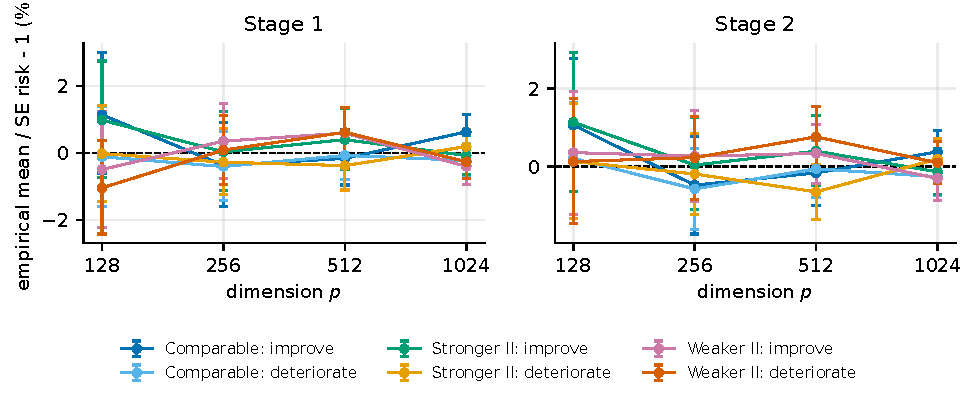
\includegraphics[width=\linewidth]{../results/publication/figures/risk_accuracy.pdf}
    \caption{Relative deviation of Monte Carlo mean risks from finite-$p$
    state-evolution risks. Error bars transform the pointwise 95\% bootstrap
    intervals for the empirical means.}
    \label{fig:se-risk-accuracy}
\end{figure}

\subsection{Matched phase test}
\label{app:numerical-validation-phase}

Let $D_p=\mathcal R_p^{(2)}-\mathcal R_p^{(1)}$, so $D_p<0$ denotes
weak-to-strong improvement. The empirical mean and state evolution agree in
sign in 24 of 24 case--dimension comparisons. The paired
pointwise 95\% interval excludes zero in 24 of 24 comparisons.
Table~\ref{tab:matched-phase-results} reports the largest dimension. At
$p=1024$, Stage II reduces the Monte Carlo mean prediction risk by
21.7\% (Comparable), 9.2\% (Stronger II), 13.1\% (Weaker II) in the
3 theory-predicted improvement regimes.

\begin{table}[t]
\centering
\caption{Matched phase test at $p=1024$. Intervals are pointwise paired 95\% percentile-bootstrap intervals for the mean risk difference.}
\label{tab:matched-phase-results}
\scriptsize
\begin{tabular}{lccc}
\toprule
Regime & $(\alpha_1,\alpha_2)$ & Empirical $D_p$ [95\% CI] & SE $D_p$ \\
\midrule
Comparable: improve & (1.25,1.25) & -0.020523 [-0.020781, -0.020269] & -0.020217 \\
Comparable: deteriorate & (1.65,1.65) & 0.000454 [0.000438, 0.000469] & 0.000457 \\
Stronger II: improve & (1.25,1.60) & -0.008633 [-0.008702, -0.008562] & -0.008593 \\
Stronger II: deteriorate & (1.65,1.70) & 0.000274 [0.000261, 0.000286] & 0.000273 \\
Weaker II: improve & (1.30,1.20) & -0.008369 [-0.008632, -0.008109] & -0.008460 \\
Weaker II: deteriorate & (1.55,1.20) & 0.016622 [0.016481, 0.016765] & 0.016566 \\
\bottomrule
\end{tabular}
\end{table}


\begin{figure}[t]
    \centering
    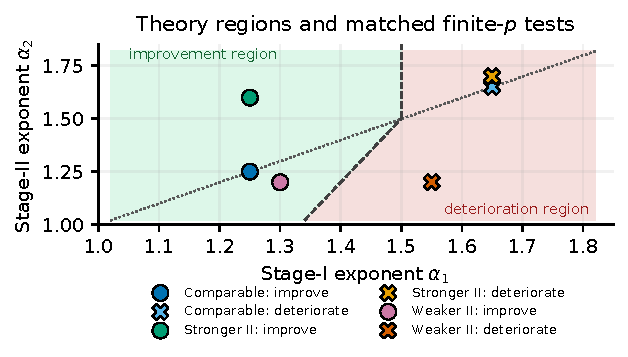
\includegraphics[width=0.72\linewidth]{../results/publication/figures/phase_diagram.pdf}
    \caption{Off-critical theoretical regions and matched empirical outcomes
    at $p=1024$. Circles denote empirical improvement and crosses denote
    deterioration.}
    \label{fig:matched-phase-diagram}
\end{figure}

\subsection{Threshold-renormalization diagnostic}
\label{app:numerical-validation-threshold}

For the scalar channels we compute
\[
Q_p=\frac1p\sum_{i=1}^p\mathbb E[(B_i-\overline B_{i,p})^2].
\]
The numerical results satisfy $Q_p\leq\sigma_{2,p}^2$ in every tested cell,
and the largest numerical error in the exact composition identity
$\eta(\eta(u;b_1);b_2)=\eta(u;b_1+b_2)$ is $2.27\times10^{-13}$.
Figure~\ref{fig:threshold-diagnostic} reports both the unnormalized
perturbation and its ratio to the Lipschitz bound for all 6 cases;
the largest ratio is 0.919. These are internal scalar-channel
checks of the deterministic composition identity and Lipschitz inequality,
not an independent coordinate-level validation of the finite-sample LASSO
mechanism. The empirical risk agreement in
Figure~\ref{fig:se-risk-accuracy} provides separate, indirect
finite-dimensional evidence for the scalar description.

\begin{figure}[t]
    \centering
    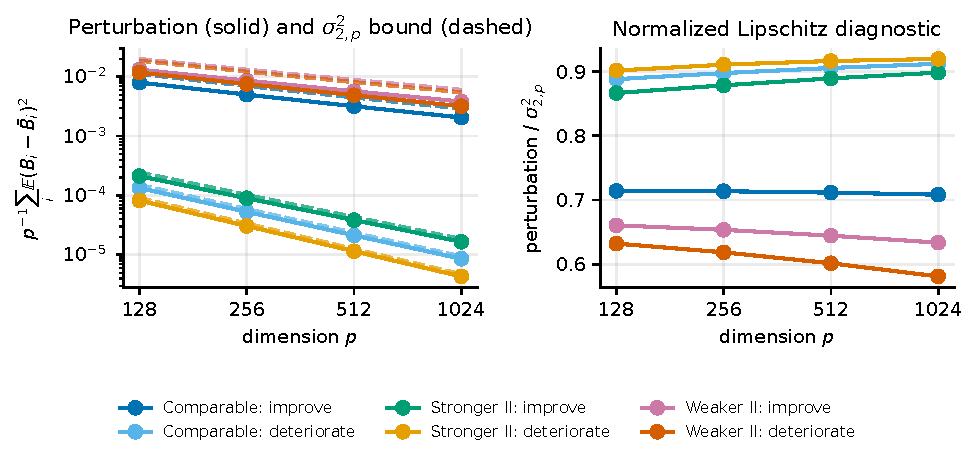
\includegraphics[width=\linewidth]{../results/publication/figures/threshold_diagnostic.pdf}
    \caption{Internal Stage-II scalar perturbation diagnostic and its
    Lipschitz bound across all 6 matched cases.}
    \label{fig:threshold-diagnostic}
\end{figure}

\subsection{Compute resources and scope}
\label{app:numerical-validation-compute}

The verified run used 6 CPU workers on an anonymized host
with an AMD EPYC 9V74 80-Core Processor CPU. Available system memory was 15.9 GiB;
no GPU was used. Python 3.12.13 and exact package versions
are recorded in the supplementary metadata. The reported run took
2.1 minutes wall-clock time and
0.16 aggregate worker-hours; maximum
recorded worker resident memory was 121
MiB. Preliminary benchmarks, unit tests, and smoke runs used less than 0.1
additional worker-hour.

The evidence is limited to $p\leq1024$, Gaussian designs, the stated power-law
signal, and selected off-critical exponent pairs and regularization constants.
It supports finite-dimensional agreement with the scalar predictions but does
not prove state evolution for the oversampled triangular array. Because the
discrepancies are not monotone in $p$, these experiments also do not establish
a convergence rate. They do not determine signs on critical boundaries or
establish transfer to nonlinear networks or real data. The reported confidence
intervals are pointwise rather than simultaneous across the 24 comparisons.
